\documentclass{article}
\usepackage{indentfirst}
\usepackage{amsmath,amsthm,amssymb}
\usepackage{mathtext}
\usepackage{amsfonts}
\usepackage[T2A]{fontenc}
\usepackage[utf8]{inputenc}
\usepackage[english]{babel}
\usepackage{graphicx}
\usepackage{hyperref}

\title{Point Generation Network in the motion command recognition task}
\author{Kseniya Shutova, Nikolay Andreychik}

\date{December 2021}

\renewcommand*\abstractname{Summary}

\begin{document}

\maketitle
\begin{abstract}

    This paper is devoted to the topic of robot recognition of motion commands. The main goal was to implement a mechanism for robot recognition of systematized commands from unstructured sources, in particular, human speech.
    
    The tasks we set for this project:
    
    \begin{enumerate}
      \item Make a dataset of possible sentences from a human to a robot, containing a veiled motion command, and target commands easily recognized by the robot.
      \item Implement an encoder that will convert an incoming sequence containing a motion command into a context vector.
      \item Implement a Point Generation Network (PGN)-based decoder to correctly fill the output command slots from the incoming sequence.
    \end{enumerate}

    You can read the program at this link: \url{https://github.com/Koolana/NLPForRobot}.
\end{abstract}


\section{Introduction}
The task of human-machine communication has interested scientists and programmers for decades. Robotic systems are entering more and more into our everyday lives. For example, autonomous robotic couriers have appeared around the world, capable of moving cargo to its destination.

We are interested in the interaction between a human and a robot courier to translate a phrase to a human into a command to move a shipment through an area whose map is already known to the robot.

The peculiarity of our task is that there are no such developments in the public domain among widely known analogues in Russian.

\subsection{Team}

\textbf{Kseniya Shutova} created a wide dataset of motion commands, developed the program code, and prepared this document.

\textbf{Nikolay Andreychik} created a neural network model to recognize motion commands, developed program code, and prepared this document.


\section{Related Work}
\label{sec:related}

\par{\cite{article_1} This project uses PGN, but the authors consider the task of compressing information. From a large amount of information make a compressed form, leaving only the main data with minimal loss of meaning.}

\cite{article_2} In this paper the authors describe a PGN-based approach for the problem of partitioning an incoming sequence into commands and their associated slots. It is noteworthy that inside the slots are words from the original sequence.

\section{Model Description}
A description of our approach.

\textbf{Task seq2seq and Attention}

By machine translation we mean any general seq2seq (sequence to sequence) problem, i.e. translation between sequences of tokens of any nature.

Encoder-Decoder is the standard modeling paradigm for sequential to sequential tasks. Its structure consists of two components:

\begin{enumerate}
\item Encoder - reads the original sequence and creates its semantic representation;
\item Decoder - uses the input semantic representation to generate the target sequence.
\end{enumerate}

Language models estimate unconditional probability $p(y)$ of sequence $y$, sequence-to-sequence models should estimate conditional probability $p(y|x)$ of sequence $y$ given source $x$. Therefore, sequence-to-sequence problems can be modeled as Conditional Language Models (CLM) - they work similarly to LMs (Language Models), but additionally obtain source information $x$.

Since the only difference from LMs is the source $x$, modeling and learning are very similar to language models. In particular, the high-level pipeline looks as follows:
\begin{enumerate}
\item feed source and previously generated target words into the network;
\item obtain a vector representation of the context (both source and previous target) from the network decoder;
\item predicting, based on this vector representation, the probability distribution for the next token.
\end{enumerate}

Like neural classifiers and language models, we can think very simply about the classification part (i.e., how to get character probabilities from a vector representation of text). The vector representation of text has some dimension $d$, but eventually we need a vector of size $|V|$ (probabilities for $|V|$ tokens/classes). To get a vector of size $|V|$ from a $d$-size vector, we can use a linear layer. Once we have a $|V|$-size vector, all that remains is to apply the softmax operation to convert the raw numbers into token probabilities.

Similar to neural LMs, seq2seq neural models are trained to predict the probability distributions of the next token given the previous context (source and previous target tokens). Intuitively, at each step we maximize the probability that the model assigns to the correct token.

Formally, we can assume that we have a training instance with initial $x = (x_1,...,x_m)$ and target $y = (y_1,...,y_n)$. Then at time step $t$ the model predicts the probability distribution
\begin{center}
$p^{(t)}=p(*|y_1,...,y_{t-1}, x_1,...,x_m)$.
\end{center}

The goal in this step is $r^* = onehot(y_t)$, i.e., we want the model to assign probability 1 to the correct token, $y_t$, and zero to the others.

The standard loss function is the cross-entropy loss. The cross-entropy loss for the target distribution $p^*$ and the predicted distribution $p$ is
\begin{center}
    $ Loss(p^*,p) = -p^*\log(p) = -\sum_{i = 1}^{|V|}p^{*}_{i} \log(p_i)$
\end{center}

Since only one of $p_{i}^{*}$ is nonzero (for the correct token $y_t$), we get
\begin{center}
    $ Loss(p^*,p) = -\log(p_{y_t}) = -\log(p(y_t|y<t,x))$
\end{center}

At each step, we maximize the probability that the model assigns the correct token.

In the models discussed above, the encoder compressed the entire source sentence into a single vector. This can be very difficult - the number of possible source values is infinite. When the encoder is forced to put all the information into one vector, it is likely to forget something.

Not only is it difficult for the encoder to put all the information into a single vector, it is also difficult for the decoder. The decoder sees only one representation of the source. However, at each stage of generation, different parts of the source may be more useful than others. But under current conditions, the decoder must extract relevant information from the same fixed representation, which is hardly easy to do.

The Attention function can be described as mapping a query and a set of key-value pairs to an output, where the query, keys, values, and output are all vectors. The output is computed as a weighted sum of values, where the weight assigned to each value is computed by the compatibility function of the query with the corresponding key.

Attention was drawn in the article "Neural Machine Translation by Jointly Learning to Align and Translate" \cite{article_3} to solve the fixed representation problem.

The Attention mechanism is part of the \ref{fig:network} neural network. At each decoding step, it decides which parts of the source are more important. In this case, the encoder does not need to compress the whole source into a single vector - it provides representations for all source tokens (e.g., for all RNN states instead of the last one).

The basic idea is that the network can learn which inputs are more important at each stage. Since everything here is differentiable (attention function, softmax, and everything else), the model with attention can be trained from start to finish. That is, we don't need to specifically teach the model to pick up the words we want; the model will learn to pick up the important information itself.

\begin{figure}[!tbh]
    \centering
    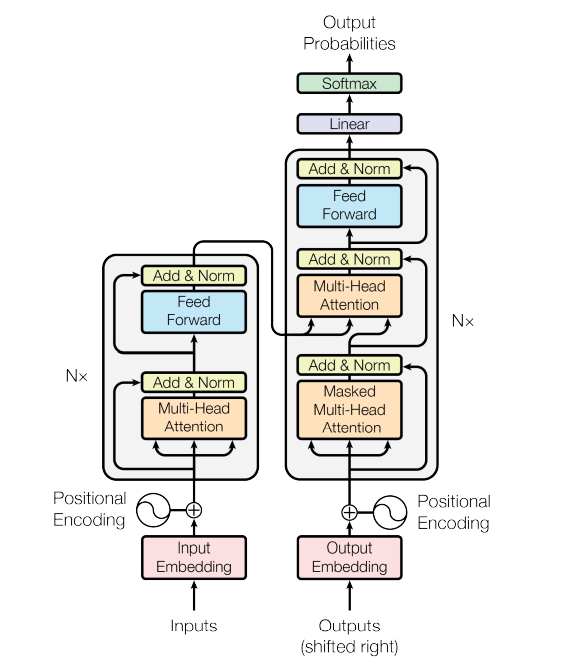
\includegraphics[width=0.7\linewidth]{network.png}
    \caption{The network architecture.}
    \label{fig:network}
\end{figure}


\textbf{Using Multi-head Attention}

Multi-head Attention allows the model to jointly process information from different subspaces of the representation in different positions. With single head Attention, averaging prevents this. 
\begin{center}
    $ MultiHead(Q,K,V) = Contact({head}_1,..., {head}_h)W^{O}$
\end{center}
где ${head}_i = Attention(Q{W}^{Q}_{i}$, $K{W}^{K}_{i}, V{W}^{V}_{i})$.
Here the projections are matrices of parameters ${W}^{Q}_{i}, {W}^{K}_{i} \in \mathbb{R}^{d_{model} \times d_k}, {W}^{V}_{i} \in \mathbb{R}^{d_{model}\times d_v}$ и  $W^O \in$ \\$\in \mathbb{R}^{hd_v\times d_{model}}$.
In the considered work, the authors use $h = 8$ parallel layers of attention, or heads. For each of them we use $d_k = _dv = d_{model}/h = 64$. Because of the reduced size of each head, the total computational cost is similar to the cost of processing a single head with full dimensionality.

An array of possible Attention Distribution points: a set of eight word importance accounts, combined by a linear neural layer \ref{fig:baseline_seq2seq_model}. For each output state, the authors count Attention for previous incoming words in latent states, that is, words that carry more semantic contribution. Based on the eight accounts, one Attention is collected. Each cell contains a word importance score for the current iteration to predict the next vector.

\begin{figure}[!tbh]
    \centering
    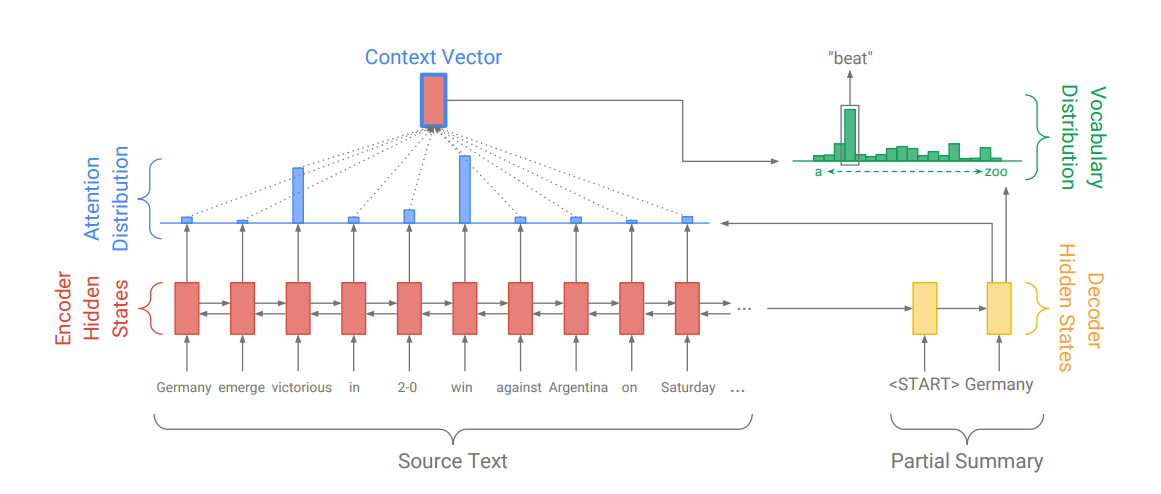
\includegraphics[width=0.9\linewidth]{baseline_seq2seq_model.png}
    \caption{Baseline sequence-to-sequence model with attention.}
    \label{fig:baseline_seq2seq_model}
\end{figure}

The model can pay attention to relevant words in the source text to create new words, for example, to create a new word beat in the abstract summary "Germany beat Argentina 2-0" the model can pay attention to the words "victorious" and "victory" in the source text.

The context vector can be transformed into the final output vocabulary distribution using a linear layer. For example, Vocabulary Distribution selects the most likely next word in the input vocabulary. In the figure, you can see what interactions happen with the final distribution (from the Attention Distribution block, the movement goes straight to Vocabulary Distribution).

\textbf{Using the Point Generation Network}

To predict the next word, an additional linear layer is introduced, which is responsible for including the distribution from the input vector dictionary. In Multi-head Attention, the distribution of the context vector was only on the output dictionary. Using the influence distribution, we can add the input dictionary to the output dictionary, thereby increasing the probable word \ref{fig:baseline_pgn} fallout.

\begin{figure}[!tbh]
    \centering
    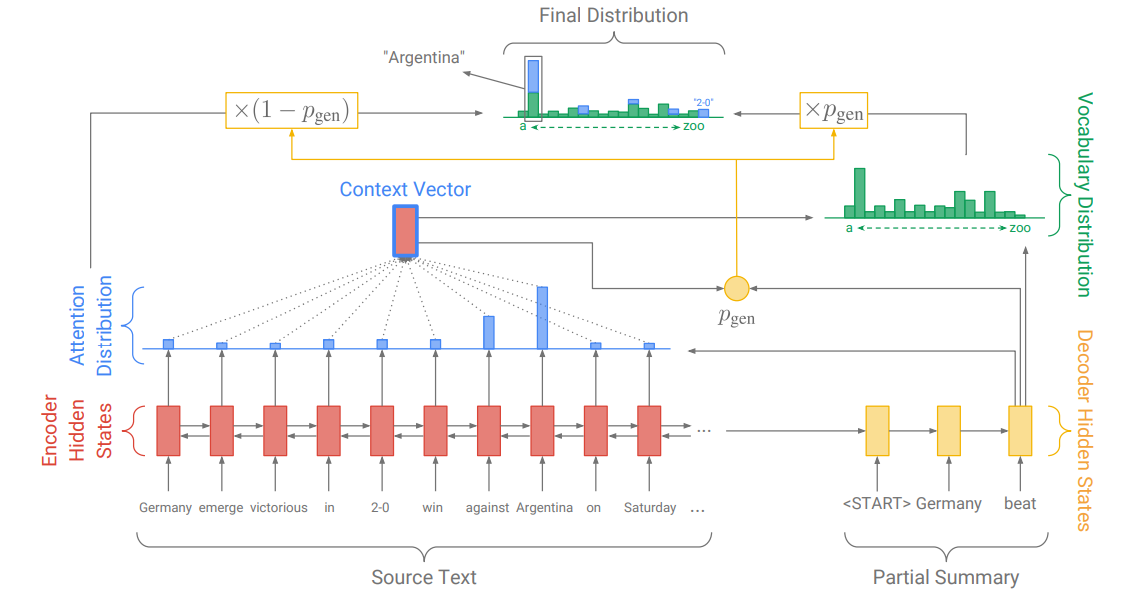
\includegraphics[width=0.9\linewidth]{baseline_pgn.png}
    \caption{Pointer-generator model.}
    \label{fig:baseline_pgn}
\end{figure}

The pointer generator network is a hybrid between baseline and pointer networks \cite{article_5}, since it allows both copying words with pointer and generating words from a fixed dictionary. In the pointer generator model \ref{fig:baseline_pgn} attention distribution $a^t$ and context vector $h^{*}_{t}$ are calculated as follows:
\begin{center}
    $a^t = softmax(e^t)$,
\end{center}
\begin{center}
    $h^{*}_{t} = sum_{i}a^{t}_{i}h_i$.
\end{center}

In addition, the generation probability $p_{gen}\in[0,1]$ for time step t is calculated from the context vector $h^{*}_{t}$, decoder state st and decoder input signal $x_t$:

\begin{center}
    $p_{gen} = \sigma(w^{T}_{h^{*}}h^{*}_{t} + w^{T}_{s}s_{t} + w^{T}_{x}x_{t} + b_{ptr})$,
\end{center}
where vectors $w_{h^{*}}, w_s, w_x$ and scalar $b_{ptr}$ are the studied parameters, and $\sigma$ is a sigmoid function.

Further, $p_{gen}$ is used as a program switch to choose between creating a word from the dictionary by sampling from $P_{vocab}$ or copying a word from the input sequence by sampling from $a^t$ Attention distribution. For each document, let the expanded dictionary denote the union of the dictionary and all the words found in the original document. We obtain the following probability distribution for the expanded dictionary:
\begin{center}
    $P(w) = p_{gen}P_{vocab}(w) + (1-p_{gen})\sum_{i: w_i = w}a^{t}_{i}$.
\end{center}
\begin{center}
    $P_{vocab} = softmax(V'(V[s_t,h^{*}_{t}]+b)+b')$,
\end{center}
where $V, V', b, b'$ are the studied parameters. $P_{vocab}$ is the probability distribution over all words in the dictionary and gives us our final distribution from which we can predict words w: $P(w) = P_{vocab}$.

During training, the loss for time step $t$ is the negative logarithmic probability of the target word $w^{*}_{t}$ for that time step: ${loss}_t = -\log{P(w^{*}_{t})}$. The total loss for the whole sequence is $loss = \frac{1}{T}\sum^{T}_{t = 0}{loss}_t$.

Note that if $w$ is a word outside the dictionary (OOV), then $P_{vocab}(w)$ is zero; similarly, if $w$ does not appear in the source document, then $\sum_{i: w_i = w}a^{t}_{i}$ is zero.

The ability to create OOV words is one of the major advantages of pointer generator models; unlike models like baseline, they are limited by their predefined vocabulary.

For each time step of the decoder, the generation probability $p_{gen} \in [0,1]$, which weights the probability of generating words from the dictionary compared to copying words from the source text. The vocabulary distribution and the attention distribution are weighted and summed to obtain the final distribution, on the basis of which the prediction is made. 

The peculiarity of this approach is that using both dictionaries increases the chance of finding the right word, without substituting synonyms from the output dictionary. For example, in this figure there is no information about the word "2-0" in the final distribution, but there is information about it in the final distribution. That is, the new added elements from the final distribution can be pulled up to the final dictionary.

\begin{figure}[!tbh]
    \centering
    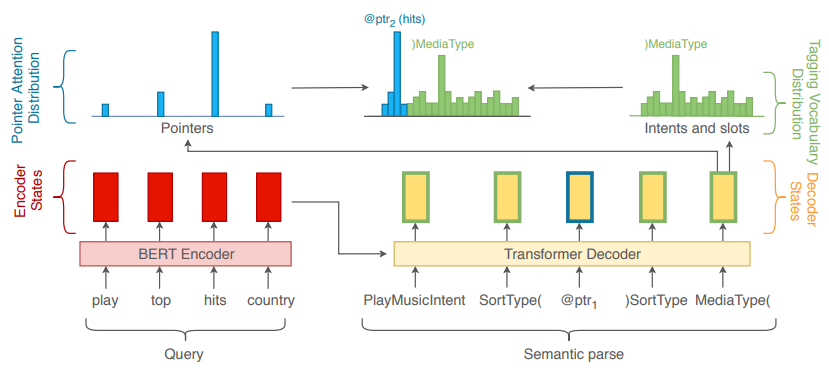
\includegraphics[width=0.9\linewidth]{Sem_parce.png}
    \caption{Sequence to Sequence model with Pointer Generator Network.}
    \label{fig:sem_parce}
\end{figure}

When converting human speech into a command for the robot, we need to preserve the meaning as much as possible and not lose the words responsible for the items to be dragged and the words responsible for the destination. That is, the information from the input sequence will be transferred to the vocabulary distribution on the output sequence to increase the probability of selecting the words of the input vocabulary. One example for our work: keeping the same cabinet number mentioned in human speech in the transformed robot command.

Our work uses dictionaries: the input sequence and the command set. This is to ensure that the output knows only the sequence of commands (move, take) and the words that come in at the input.

The article \cite{article_4} deals with the transformer with a dictionary consisting only of the slot command, which includes a single word inside it. In our case, the slot will be the "take" command. Inside the slot must be words taken not from the dictionary, but from Pointer Attention Distribution \ref{fig:sem_parce}.

The model currently predicts the token after "MediaType(" by looking at the tag dictionary scores and attention by source pointers. It generates "@ptr2" because it has the highest overall score.

\section{Dataset}
In this modification of the program we have 3 kinds of commands for the robot:

\begin{itemize}
  \item взять (ОБЪЕКТ) взять движение (ПУНКТ НАЗНАЧЕНИЯ) движение.
  
  This command involves loading and transferring an object from the current point A to point B.
  
  Example: 
  
  Input sequence: 'не откажи в любезности прихватить весы в библиотеку пожалуйста'
  
  Translation of text to the command: 'взять (весы) взять движение (библиотека) движение'
  
  \item движение (ПУНКТ НАЗНАЧЕНИЯ) движение взять (ОБЪЕКТ) взять движение (ОБРАТНО) движение.
  
  This command involves moving from point A to point B, loading the object at that point, and moving back to point A with the object.
  
  Example: 
  
  Input sequence: 'доберись пожалуйста в буфет и довези мне книжку'
  
  Translation of text to the command: 'движение (буфет) взять (книжка) взять движение (обратно) движение'
  
  \item взять (ОБЪЕКТ) взять движение (ПУНКТ НАЗНАЧЕНИЯ) движение движение (ОБРАТНО) движение.
  Данная команда подразумевает погрузку объекта в пункте А, движение в пункт В, выгрузку объекта и движение обратно в пункт А.
  
  Example:
  
  Input sequence: 'привет отвези объект в библиотеку затем дойди обратно'
  
  Translation of text to the command: 'взять (объект) взять движение (библиотека) движение движение (обратно) движение'
\end{itemize}

Dataset is based on a random selection of sentences from 86 possible command patterns. 

An array of subjects is generated from a set of 50 thousand words of Russian nouns. This is necessary so that the neural network does not get hung up on a particular object.

Each pattern is fed with different words that are responsible for certain contexts.
For example, we can generate a sentence with a polite (пожалуйста, будь добр) or demanding (сию минуту, немедленно) tone, with or without a greeting, with an additional specification (привезти только для меня или только сюда или только этот предмет, etc.). It is also possible to specify who exactly is asking the robot to bring or take away this or that thing (я хочу, мы хотим, она просит, он желает, etc.).

The sentences have varying degrees of complexity. It can be a simple command ("принеси из библиотеки книгу"), or it can be a more complex sentence with an implicit command ("доброе утро Полине охота чтобы ты прихватил пицца в кампус Африка").

The challenge is that, regardless of the complexity of the offer, the agent recognizes what he needs to take, where to take it, and what to do next.

You can read the dataset generator at the following link: \url{https://github.com/Koolana/NLPForRobot/blob/main/src/generatorSentence.py}

To get the generated sample, write the following command: generateSent(N), where N is the number of sentences for the dataset. Our data is cleaned from repeating sentences and from extra spaces. The generated data is stored in the datasets folder.

\begin{figure}[!tbh]
    \centering
    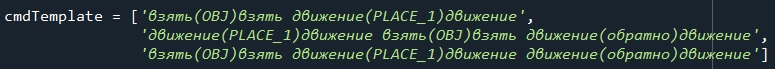
\includegraphics[width=1\linewidth]{cmdTemplate.jpg}
    \caption{Classes of commands handled by the robot.}
    \label{fig:cmdTemplate}
\end{figure}
\begin{figure}[!tbh]
    \centering
    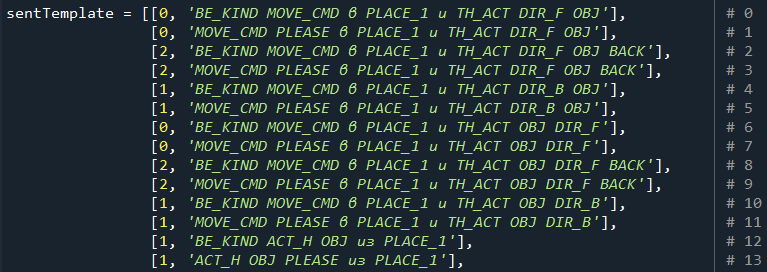
\includegraphics[width=0.9\linewidth]{sentTemplate.png}
    \caption{Command templates that represent a sentence with a direct command to the robot.}
    \label{fig:sentTemplate}
\end{figure}
Let's take a closer look at this program. Figure \ref{fig:cmdTemplate} shows the classes of commands to be received after the processing of the intended human task. Figure \ref{fig:sentTemplate} shows the first 13 human speech patterns.
The word arrays for generating sentences based on the templates are stored in vectors. At each iteration, the sets of words in a sentence are randomly generated sequentially according to the template currently under consideration.

Generation is performed in the part of the program below the figure \ref{fig:main_part}.
\begin{figure}[!tbh]
    \centering
    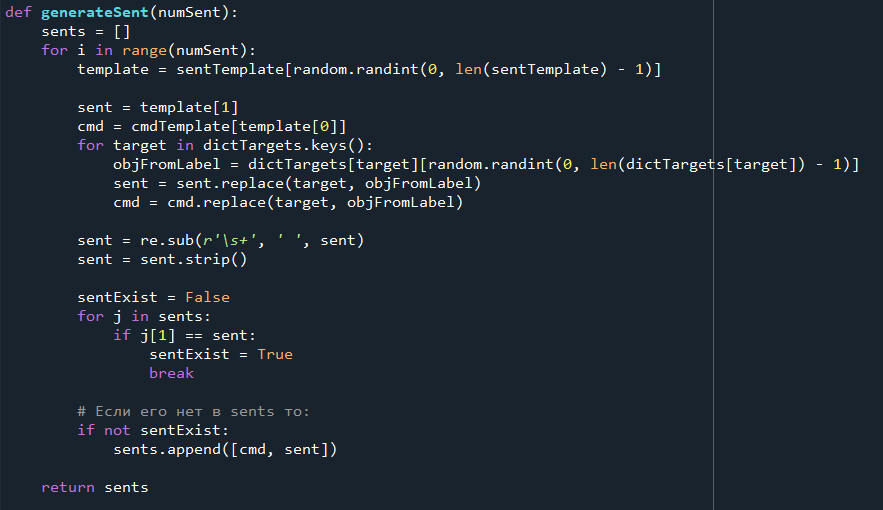
\includegraphics[width=0.9\linewidth]{main_part.png}
    \caption{Command templates representing a sentence with a direct command to the robot.}
    \label{fig:main_part}
\end{figure}

\begin{itemize}
\item sents -- array, which will store all human commands to the robot.
\item numSent -- the desired number of generated commands
\item template is the template under consideration, by which the command will be built. It has the form: [index, command].
\item cmd = cmdTemplate[template[0]] -- a direct command readable in the robot's language. Such a command corresponds to an index in template.
\item dictTarget -- elements that represent a reference to a specific word array. The dictTarget combination specifies a sentence.
\item sent -- in the for loop into this array, the words at each position in dictTarget are randomly generated starting from the last element of the pattern.
\item cmd -- in cmd as well as in sent the words for the final command to the robot are sequentially generated.
\end{itemize}


\section{Experiments}

\subsection{Metrics}
To evaluate our model, we used the BLEU metrics (unigrams, bigrams, trigrams, four-grams) и ACCURACY.

$$BLEU(N) = BP \cdot GAPS(N),$$
where $BP = \begin{cases}
   1 &\text{$c \geq r $}\\
   \exp(1 - \frac{r}{c})  &\text{$c<r$}
 \end{cases}$, and $GAPS = \exp(\sum \omega_n \log(P_n))$

\begin{itemize}
\item BP - Brevity Penalty

\item GAPS - Geometric Average Precision Scores
\end{itemize}

\subsection{Experiment Setup}

Our model was trained on a GP107M [GeForce GTX 1050 Mobile] with 2GB of video memory without a pre-trained encoder on 50 epochs. The set of input sequences was preliminarily cleaned from punctuation marks and the BPE tokenizer of the ruRoberta model from SberDevices team was chosen as the tokenizer.

The following hyperparameters were set in our model:
\begin{itemize}
\item HID\_DIM = 256 - dimension of the hidden state vector
\item ENC\_PF\_DIM = 512 - hidden units encoder
\item DEC\_PF\_DIM = 512 - hidden units decoder
\item ENC\_LAYERS = 3 - number of layers encoder
\item DEC\_LAYERS = 3 - number of layers decoder
\item ENC\_HEADS = 8 - number of heads multi-head attention encoder
\item DEC\_HEADS = 8 - number of heads multi-head attention decoder
\end{itemize}

Train and validation data was generated in the ratio of 80\% to 20\% of the total dataset, test data - separately, not related to the previous dataset in the amount of 10\% of the training data. It is on the test data that the above mentioned metrics were calculated.

The cross entropy function was used as the loss function, and Adam with learning rate 5e-4 as the optimizer.

\subsection{Baselines}
There is a model Shift Reduce Parser, which can be used to perform rule-based sentence parsing, without the use of neural networks. This paper did not analyze its accuracy on our generated dataset, but on similar datasets for English, it is about 0.8.

\section{Results}

The following results were obtained for our model on the self-generated test sample (Table \ref{tab:results}):
\begin{table}[!tbh]
\begin{center}
\begin{tabular}{ | l | l | l | }
\hline
\textbf{METHOD} & \textbf{BLEU} & \textbf{ACCURACY} \\ \hline
ruSeq2Seq-Ptr & 98.6 & 81.2 \\
\hline
\end{tabular}
\caption{Metrics results.}
\label{tab:results}
\end{center}
\end{table}

\begin{table}[!tbh]
\begin{center}
\begin{tabular}{ | l | l | l | }
\hline
\textbf{METHOD}  & \textbf{ACCURACY} & \textbf{DATASET}\\ \hline
Shift Reduce (SR) Parser & 80.86 & Facebook Top \\
SR with ELMo embeddings & 83.93 & Facebook TOP \\
SR ensemble + ELMo + SVMRank & 87.25 & Facebook TOP \\
Joint BiRNN & 80.70 & ATIS \\
Attention BiRNN & 78.90 & ATIS \\
Slot Gated Full Attention & 82.20 & ATIS \\
CapsuleNLU & 83.40 & ATIS \\
\hline
\end{tabular}
\caption{Other methods.}
\label{tab:methods}
\end{center}
\end{table}

Making a direct comparative analysis with other approaches is difficult, since the vast majority of datasets for our problem have been created under the condition of using the English language. Below we provide the results (Table \ref{tab:methods}) of similar works on the subject, through which our approach can be indirectly analyzed. As can be noted, our model has acceptable accuracy in this problem.

\begin{table}[!tbh]
\begin{center}
\begin{tabular}{ | p{5cm} | p{6cm} |}
\hline
\textbf{Input sentence}  & \textbf{Predicted command} \\ \hline
<s> не сочтите за труд привезти кружку из медпункт пожалуйста </s> & <s> движение( мед п ункт )движение взять( к руж ку )взять движение(обратно)движение </s> \\
\hline
<s> принеси чашку из кабинет 345 </s> & <s> движение( каб инет 3 45 )движение взять( ч ашку )взять движение(обратно)движение </s> \\
\hline
<s> переместись пожалуйста в библиотеку и отнеси им блокнот </s> & <s> взять( бл ок нот )взять движение( б иблиот еку )движение </s> \\
\hline
<s> отнеси посуду на склад </s> & <s> взять( пос уду )взять движение( на ск лад )движение </s> \\
\hline
\end{tabular}
\caption{Inputs and predicted commands}
\label{tab:methods}
\end{center}
\end{table}



\section{Conclusion}
According to the results of this work we have implemented a data generator, which allows to generate dataset on the basis of 86 templates for 3 types of commands. A dataset of size 50 thousand pairs was generated (input sequence - command), a test dataset of size 5 thousand pairs with the help of our dataset generator. 

We developed a model for semantic analysis of the input sequence based on Point Generation Network, which allows to generate the output command by relying on the input sequence through pointers to words, keeping the necessary data (such as numbers of cubicles, sites and so on). Ultimately, the resulting model showed acceptable accuracy in recognizing command objects compared to other methods. 

\bibliographystyle{apalike}
\bibliography{lit}
\end{document}

